\documentclass[conference]{IEEEtran}
\IEEEoverridecommandlockouts
% The preceding line is only needed to identify funding in the first footnote. If that is unneeded, please comment it out.
\usepackage{cite}
\usepackage{amsmath,amssymb,amsfonts}
\usepackage{algorithmic}
\usepackage{graphicx}
\usepackage{textcomp}
\usepackage{verbatim}
\usepackage{siunitx}
\usepackage{xcolor}
\def\BibTeX{{\rm B\kern-.05em{\sc i\kern-.025em b}\kern-.08em
    T\kern-.1667em\lower.7ex\hbox{E}\kern-.125emX}}
\begin{document}

\title{MECH0010 Assignment Report 1 - Group 13
}

\author{\IEEEauthorblockN{Hasha Dar}
\and
\IEEEauthorblockN{Christopher Tawk}
\and
\IEEEauthorblockN{Xichen Yang}
}

\maketitle
\begin{abstract}
    3D printers allow the rapid development of CAD modelled objects. 3D printers are also very versatile, being able to print a wide range of materials and at varying resolutions and sizes. This paper will look at the control systems and some of the measurement systems employed by 3D printers.
\end{abstract}

\section*{Introduction}
In this paper, we shall be investigating velocity and position control of a servo using Simulink, relating to the motion of the printer head. We shall also investigate circuits and design systems to measure the position of the printer head to a suitable degree of accuracy. 

\section*{Question 1 - Implement open and closed loop velocity and position control...}
In the real world, the operation of DC motor is the transfer from electrical energy to the mechanical rotation of motor. Therefore, the electric circuit of motor operation is composed by the input voltage ($v$ (\si{\volt})), terminal resistance ($R$ (\si{\ohm})), Inductance ($L$ (\si{\henry})), and the electromotive force ($em$ (\si{\volt})). In this case the formulas for the time domain and frequency domain are ($i$ is the current of the circuit):
\begin{align}
    V &= Ri + L \frac{\textrm{d}i}{\textrm{d} t} + em\\
    V(s) &= RI(s) + LsI(s) + Em(s) \label{ll1}
\end{align}
For the mechanical rotation, the relationship among torque ($T$ (\si{\newton\metre})), moment of inertia ($Im$ (\si{\kg\metre\squared})), angular displacement ($\theta$) and the friction coefficient ($b$) in time domain and frequency domain are given:
\begin{align}
    T &= Im \frac{\textrm{d}^2 \theta}{\textrm{d} t^2} + b \frac{\textrm{d} \theta}{\textrm{d} t}\\
    T(s) &= Ims^2 \theta(s) + bs\theta(s)\label{ll2}
\end{align}
In this case, angular velocity is proportional to the electromotive force and current is proportional to the torque of the motor. ($K_e$ the electrical motor constant, $K_t$ is the mechanical motor constant):
\begin{align}
    em &= K_e \frac{\textrm{d} \theta}{\textrm{d} t}\\
    Em(s) &= K_e s \theta(s)\\ \label{ll3}
    T &= K_t i\\
    T(s) &= K_t I(s) \label{ll4}
\end{align}
To find the response between angular position ($\theta$) and input voltage ($v$) in time domain, the Laplace transfer function by combination of Eq.\ref{ll1}, \ref{ll2}, \ref{ll3}, \ref{ll4} is shown below:
\begin{align}
    \frac{\theta (s)}{v(s)} = \frac{K_t}{bR_s (\frac{K_e K_t}{bR}) + \tau_e \tau_m s^2 + \tau_m s + \tau_e s +1}
\end{align}
Note: $\tau_m$ is the mechanical time constant of motor ($\tau_m=\frac{Im}{b}$), $\tau_e$ is the electrical time constant ($\tau_e=\frac{L}{R}$).

Assumption: Because the electrical time constant ($\tau_e$) is much smaller compared to the mechanical time constant of the motor ($\tau_m$), term $\tau_e\tau_ms^2$ and $\tau_es$ are approximately equal to zero compared with other terms. Therefore, the equation will become:
\begin{align}
    \resizebox{.43 \textwidth}{!}
    {$
    \frac{\theta (s)}{v(s)} = \frac{K}{s(\tau s + 1)} \ \left( K = \frac{K_t}{bR + K_t K_e}, \ \tau = \frac{\tau_m Rb}{K K_t + Rb} \right)
    $}
\end{align}
Due to the angular velocity ($\omega$) is the first derivative of angular position related to time ($\omega\left(s\right)=s\cdot\theta\left(s\right)$). In this case, the transfer function of angular velocity and input voltage is:
\begin{align}
    \frac{\omega(s)}{v(s)} = \frac{k}{\tau s + 1}
\end{align}
According to the specification data of Motor C42-L50 winding code 10 
\begin{table}[htbp]
    \caption{Specification Data}
    \begin{center}
    \begin{tabular}{|c|c|}
    \hline
    \textbf{Specification} & \textbf{Value}\\
    \hline
    \hline
    Torque sensitivity ($K_t$) & \SI{0.1412}{\newton\metre\per\ampere}\\
    \hline
    Back e.m.f. ($K_e$) & \SI{0.1413}{\volt\per\radian\per\second}\\
    \hline
    Rotor inertia ($Im$) & \SI{6.3354e-4}{\kg\per\meter\squared}\\
    \hline
    Mec. time constant ($\tau_m$) & \SI{0.0223}{\second}\\
    \hline
    Terminal resistance ($R$) & \SI{0.7}{\ohm}\\
    \hline
    Friction coefficient $\left(\frac{I_m}{\tau_m}\right)$ & \SI{0.0285}{}\\
    \hline
    \end{tabular}
    \label{sdtable}
    \end{center}
\end{table}
Therefore, the constant $K$ and overall time constant $\tau$ can be calculated as:
\begin{align}
    K = \frac{K_t}{bR + K_t K_e} &= 3.54\\ 
    \tau = \frac{\tau_m Rb}{K K_t + Rb} &= 0.0112
\end{align}
In this case, the transfer function of angular velocity and angular displacement of motor with voltage input is:
\begin{align}
    \frac{\omega (s)}{v(s)} = \frac{K}{(\tau s +1)} &= \frac{3.54}{0.0112s + 1}\\
    \frac{\theta (s)}{v(s)} = \frac{K}{s(\tau s + 1)} &= \frac{3.54}{0.0112s^2 + s}
\end{align}
where 3.54 is the gain of the system.
\begin{figure}[htbp]
    \centering
    \begin{minipage}[b]{0.24\textwidth}
        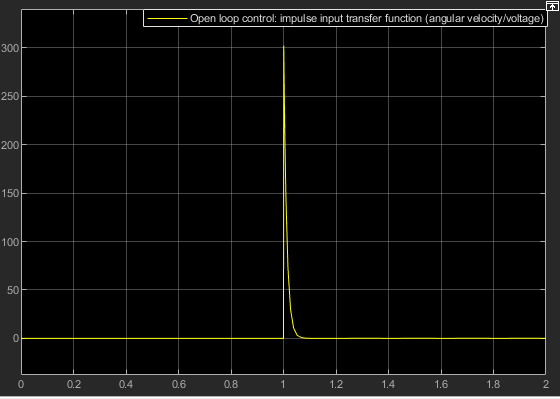
\includegraphics[width=\textwidth]{./Graph/G1.png}
        \caption{Results analysis: the response can reach desired target exponentially without oscillation.}
    \end{minipage}
    \hfill
    \begin{minipage}[b]{0.24\textwidth}
        \centering
        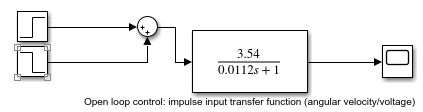
\includegraphics[width=\textwidth]{./Graph/Graph1.png}
        \caption{Model of open loop transfer function of angular velocity with impulse input.}
    \end{minipage}
\end{figure}
\begin{figure}[htbp]
    \centering
    \begin{minipage}[b]{0.24\textwidth}
        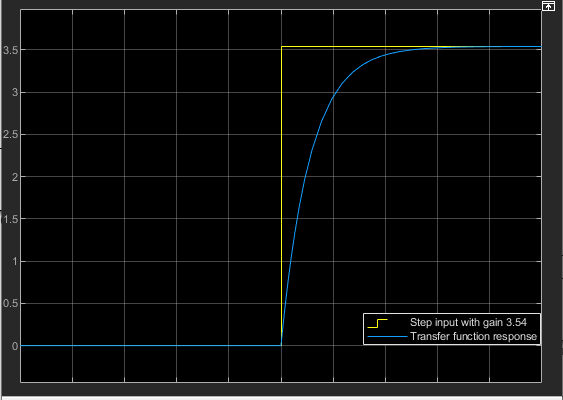
\includegraphics[width=\textwidth]{./Graph/G2.png}
        \caption{Results analysis: the response can reach desired step input exponentially without oscillation.}
    \end{minipage}
    \hfill
    \begin{minipage}[b]{0.24\textwidth}
        \centering
        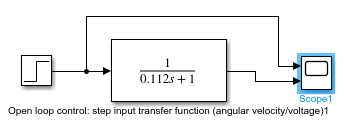
\includegraphics[width=\textwidth]{./Graph/G2'.png}
        \caption{Model of open loop transfer function of angular velocity with step input.}
    \end{minipage}
\end{figure}
\begin{figure}[htbp]
    \centering
    \begin{minipage}[b]{0.24\textwidth}
        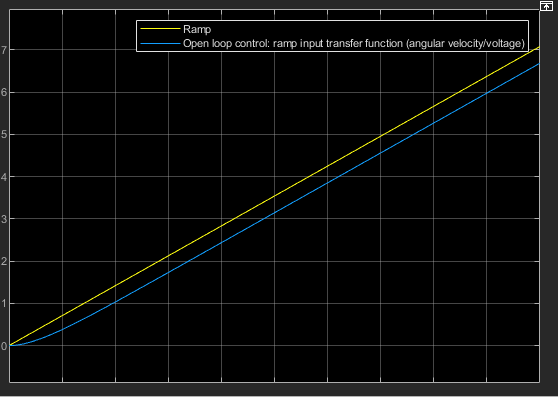
\includegraphics[width=\textwidth]{./Graph/G3.png}
        \caption{Results analysis: the response cannot reach the desired input and has a steady state lag.}
    \end{minipage}
    \hfill
    \begin{minipage}[b]{0.24\textwidth}
        \centering
        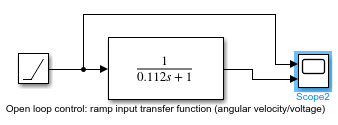
\includegraphics[width=\textwidth]{./Graph/G3'.png}
        \caption{Model of open loop transfer function of angular velocity with ramp input.}
    \end{minipage}
\end{figure}
\begin{figure}[htbp]
    \centering
    \begin{minipage}[b]{0.24\textwidth}
        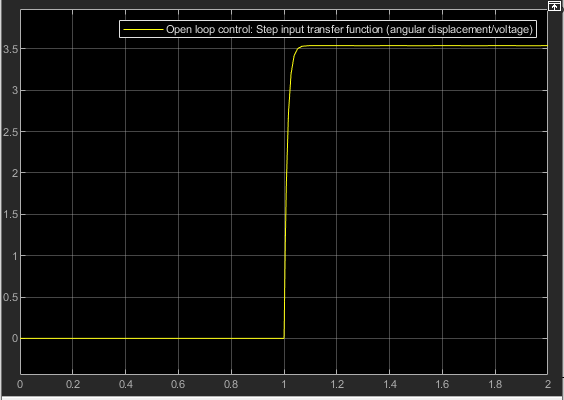
\includegraphics[width=\textwidth]{./Graph/G4.png}
        \caption{}
        \label{oltad1}
    \end{minipage}
    \hfill
    \begin{minipage}[b]{0.24\textwidth}
        \centering
        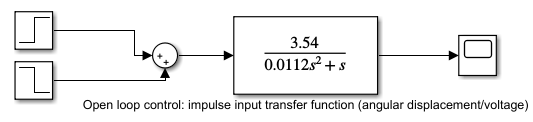
\includegraphics[width=\textwidth]{./Graph/G4'.png}
        \caption{Model of open loop transfer function of angular displacement with impulse input.}
    \end{minipage}
\end{figure}
\begin{figure}[htbp]
    \centering
    \begin{minipage}[b]{0.24\textwidth}
        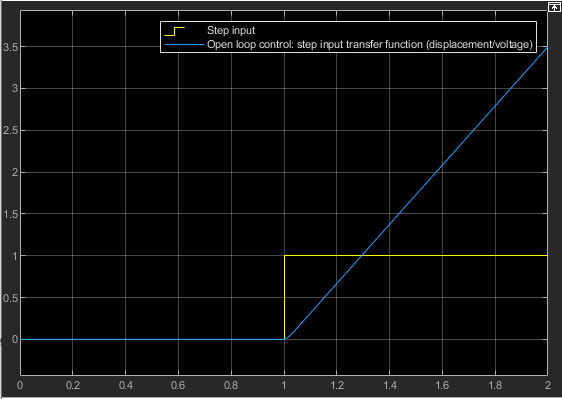
\includegraphics[width=\textwidth]{./Graph/G5.png}
        \caption{}
        \label{oltad2}
    \end{minipage}
    \hfill
    \begin{minipage}[b]{0.24\textwidth}
        \centering
        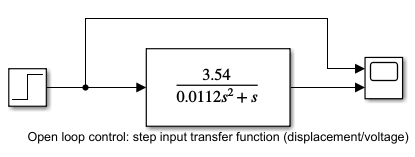
\includegraphics[width=\textwidth]{./Graph/G5'.png}
        \caption{Model of open loop transfer function of angular displacement with step input.}
    \end{minipage}
\end{figure}
\begin{figure}[htbp]
    \centering
    \begin{minipage}[b]{0.24\textwidth}
        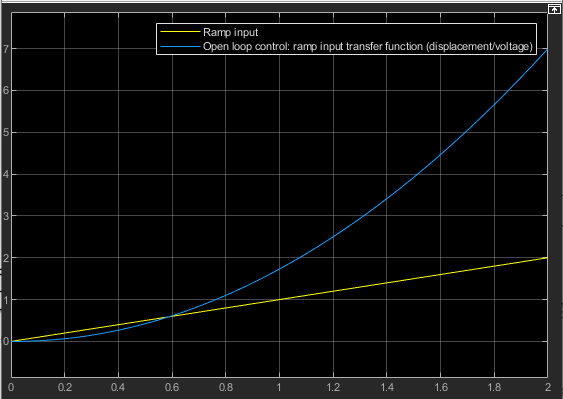
\includegraphics[width=\textwidth]{./Graph/G6.png}
        \caption{}
        \label{oltad3}
    \end{minipage}
    \hfill
    \begin{minipage}[b]{0.24\textwidth}
        \centering
        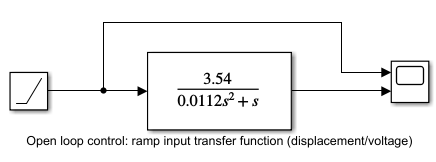
\includegraphics[width=\textwidth]{./Graph/G6'.png}
        \caption{Model of open loop transfer function of angular displacement with ramp input.}
    \end{minipage}
\end{figure}
\begin{comment}
\begin{figure}[htbp]
    \centerline{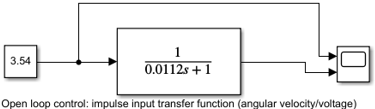
\includegraphics[width = 0.4\textwidth]{../img/q1-2.png}}
    \caption{Model of open loop transfer function of angular velocity.}
\end{figure}
\begin{figure}[htbp]
    \centerline{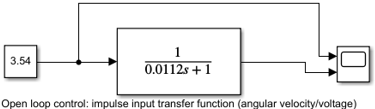
\includegraphics[width = 0.4\textwidth]{../img/q1-2.png}}
    \caption{Model of open loop transfer function of angular displacement.}
\end{figure}
\begin{figure}[htbp]
    \centering
    \begin{minipage}[b]{0.24\textwidth}
      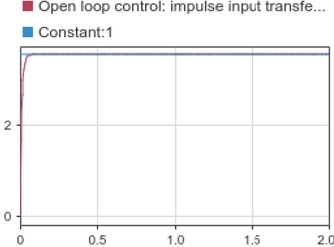
\includegraphics[width=\textwidth]{../img/q1-1.png}
      \caption{Model of open loop transfer function of angular velocity with impulse input.}
    \end{minipage}
    \hfill
    \begin{minipage}[b]{0.24\textwidth}
      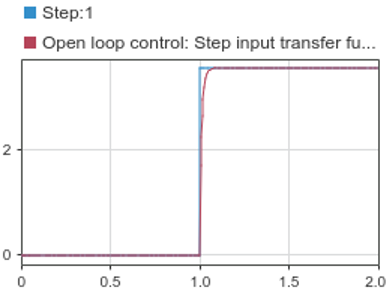
\includegraphics[width=\textwidth]{../img/q1-3.png}
      \caption{Model of open loop transfer function of angular velocity with step input.}
    \end{minipage}
\end{figure}
\begin{figure}[htbp]
    \centering
    \begin{minipage}[b]{0.24\textwidth}
      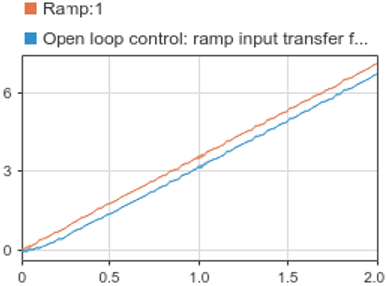
\includegraphics[width=\textwidth]{../img/q1-5.png}
      \caption{Model of open loop transfer function of angular velocity with ramp input.}
    \end{minipage}
    \hfill
    \begin{minipage}[b]{0.24\textwidth}
      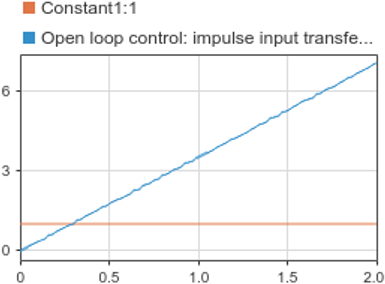
\includegraphics[width=\textwidth]{../img/q1-7.png}
      \caption{Model of open loop transfer function of angular displacement with impulse input.}
      \label{oltad1}
    \end{minipage}
\end{figure}
\begin{figure}[htbp]
    \centering
    \begin{minipage}[b]{0.24\textwidth}
      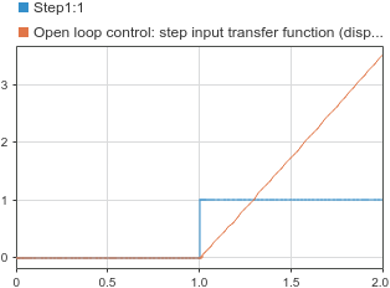
\includegraphics[width=\textwidth]{../img/q1-9.png}
      \caption{Model of open loop transfer function of angular displacement with step input.}
      \label{oltad2}
    \end{minipage}
    \hfill
    \begin{minipage}[b]{0.24\textwidth}
      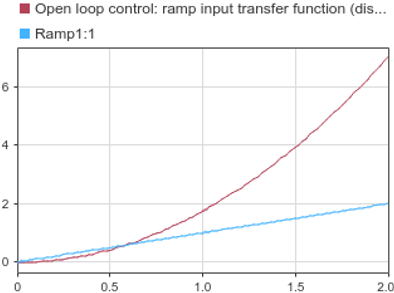
\includegraphics[width=\textwidth]{../img/q1-10.png}
      \caption{Model of open loop transfer function of angular displacement with ramp input.}
      \label{oltad3}
    \end{minipage}
\end{figure}
\end{comment}

According to the results show in Graphs.\ref{oltad1}, .\ref{oltad2}, .\ref{oltad3}, the response of output angular displacement will intersect with input and then overshoot to infinity (undesirable behaviour), which means these open loops cannot meet the requirement to control the angular displacement of the motor. Under this circumstance, the unit feedback closed loop with a gain of $H$ is required to overcome this undesirable behaviour of open loop control system for angular velocity. The formula for the feedback loop is:
\begin{align}
    G(s) &= \frac{\theta (s)}{v(s)} = \frac{3.54}{0.0112s^2 + s}\\
    H(s) &= H\\
    G'(s) &= \frac{G(s)}{1 + G(s) \cdot H(s)}
\end{align}
Therefore, the new transfer function is:
\begin{align}
    G'(s) &= \gamma \frac{\omega_n^2}{s^2 + 2\zeta \omega_n s + \omega_n^2}
\end{align}
\begin{align}
    \resizebox{.43 \textwidth}{!}
    {$
    G'(s) = \frac{316.07H}{H\left( s^2 + 2 \cdot 44.64 \cdot \sqrt{\frac{1}{316.07H}} \cdot \sqrt{316.07 H} s + 316.07 H\right)}
    $}
\end{align}
Note: $\gamma = \frac{1}{H}$, $\zeta = 44.64 \sqrt{\frac{1}{316.07H}}$ and $\omega_n = \sqrt{316.07H}$

In this case, we can use $\zeta$ to determine the response wanted as overdamped, critically damped, underdamped or undamped to control the loop without undesired behaviour, and the table below shows the range of H for the overdamped, critically damped, underdamped or undamped response cases: 
\begin{table}[htbp]
    \caption{Transfer function responses}
    \begin{center}
    \begin{tabular}{|c|c|c|}
    \hline
    \textbf{Response} & \textbf{Value of $\zeta$} & \textbf{Value of gain $H$}\\
    \hline
    \hline
    Critical damping & $\zeta > 1$ & $ 0< H < 6.304$\\
    \hline
    Overdamped & $\zeta = 1$ & $H=6.304$\\
    \hline
    Underdamped & $0<\zeta<1$ & $H > 6.304$\\
    \hline
    Undamped & $\zeta = 0$ & $H = \infty$\\
    \hline
    \end{tabular}
    \label{tfrtable}
    \end{center}
\end{table}
Therefore, the transfer function of unit feedback loop is:
\begin{align}
    G(s) = \frac{3.54}{0.0122s^2 + s}
    \label{tf}
\end{align}

The unit feedback loop servo control system is type 1 system $(P=1)$, which means there is no steady state position error for the step input and there must be a steady velocity lag for the ramp input.

For the impulse input, we want the response reach desired value fast without any oscillation, which refers to the overdamped case. Hence, H=6.304 for the impulse input situation. The Simulink model of impulse input of closed loop transfer response is shown in Graph 7.
For the step input situation, underdamped response has the fastest speed to reach the desired input value. In our case, the desired overshoot percentage is 5\%, which means our servo system can reach desired position within 5\% overshoot. Therefore, gain H can be calculated by:
\begin{align}
    \frac{A}{100} = e^{\frac{-\zeta \pi}{\sqrt{1-\zeta^2}}} = 0.05, \ \zeta = 0.69
\end{align}
In this case, $H = 13.24$ for the step input situation according to $(\zeta = 44.64 \sqrt{\frac{1}{316.1H}})$. Simulink model of step input of closed loop transfer response is shown in Fig.\ref{StepInputClosedLoopTR}. For the ramp input, there must be a steady state velocity lag due to type 1 system $(P=1)$, therefore, for better performance, we set the lag to \SI{0.1}{\second}. In this case, $H$ can be calculated by the formula:
\begin{align}
    e = \frac{a}{kv} \ (kv = \lim_{s \rightarrow 0} G(s) H(s))
\end{align}
Hence, $H=\frac{1}{e \times 3.54} = 2.82$ for \SI{0.1}{\second} velocity lag, which means the response is critical dump case. Simulink model of ramp input of closed loop transfer response in Fig.\ref{RampInputClosedLoopTR}
\begin{figure}[htbp]
    \centering
    \begin{minipage}[b]{0.24\textwidth}
        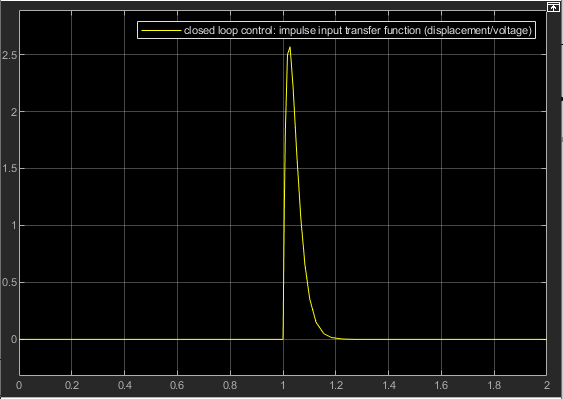
\includegraphics[width=\textwidth]{./Graph/G7'.png}
        \caption{}
    \end{minipage}
    \hfill
    \begin{minipage}[b]{0.24\textwidth}
        \centering
        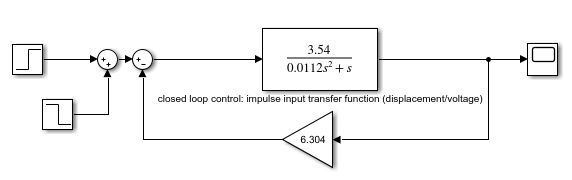
\includegraphics[width=\textwidth]{./Graph/G7.png}
        \caption{}
    \end{minipage}
\end{figure}
\begin{figure}[htbp]
    \centering
    \begin{minipage}[b]{0.24\textwidth}
        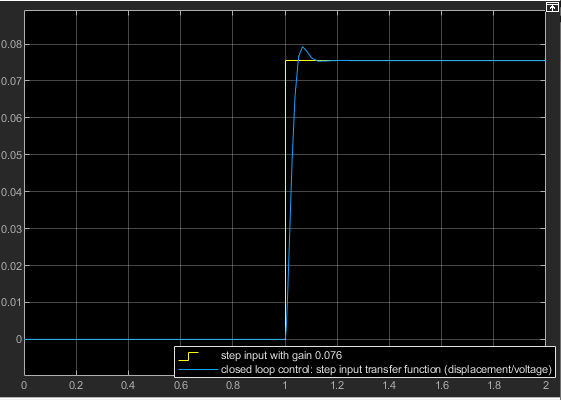
\includegraphics[width=\textwidth]{./Graph/G8.png}
        \caption{}
        \label{StepInputClosedLoopTR}
    \end{minipage}
    \hfill
    \begin{minipage}[b]{0.24\textwidth}
        \centering
        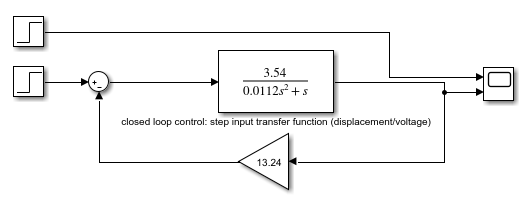
\includegraphics[width=\textwidth]{./Graph/G8'.png}
        \caption{}
    \end{minipage}
\end{figure}
\begin{figure}[htbp]
    \centering
    \begin{minipage}[b]{0.24\textwidth}
        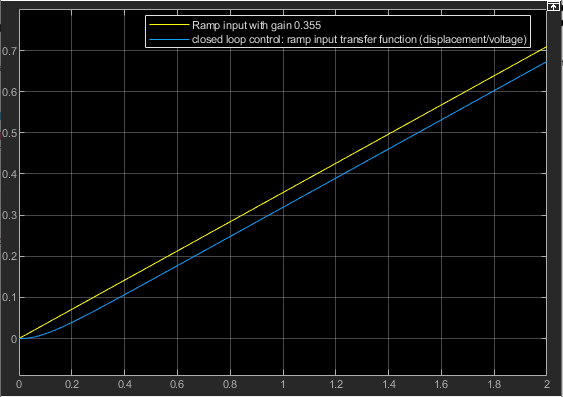
\includegraphics[width=\textwidth]{./Graph/G9.png}
        \caption{}
        \label{RampInputClosedLoopTR}
    \end{minipage}
    \hfill
    \begin{minipage}[b]{0.24\textwidth}
        \centering
        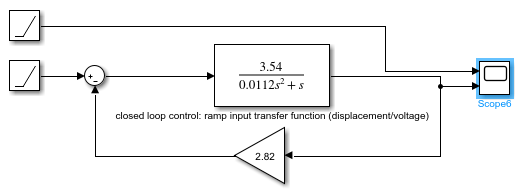
\includegraphics[width=\textwidth]{./Graph/G9'.png}
        \caption{}
    \end{minipage}
\end{figure}
\section*{Question 2}
\subsection*{2.1 - Create a light-sensing circuit...}
Building the voltage divider circuit in TinkerCAD, the light level slider was moved left and right and the range of voltages displayed were \SI{1.49}{\volt} - \SI{0.504}{\volt}. Using the formula:
\begin{align}
    V_{meter} &= \frac{R_{LDR}}{R_{R} + R_{LDR}} \times V_{in}\\
    R_{LDR} &= \frac{V_{meter}R_{R}}{V_{in} - V_{meter}}\\
    R_{LDR,max} &= \frac{1.49\times 1000}{1.5-1.49} = \SI{149e3}{\ohm}\\
    R_{LDR,min} &= \frac{0.504\times 1000}{1.5 - 0.504} = \SI{506.02}{\ohm}
\end{align}
\begin{figure}[htbp]
    \centerline{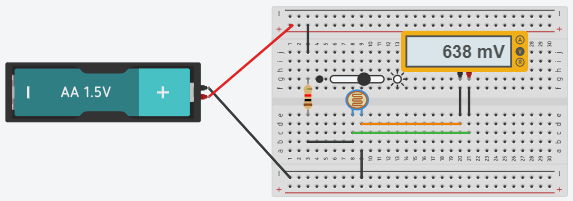
\includegraphics[width = 0.45\textwidth]{q2-1BreadBoard.png}}
    \caption{LDR on breadboard.}
\end{figure}
\subsection*{2.3 - Investigate linear position transducers...}
To measure the position of the printer head, we can utilise a variety of sensors. Some technologies that have been used to measure the position of the printer head \cite{b2}. They are:

A microswitch placed at the "home" position. This is actuated when the printer head is at the origin coordinate, hence the printer head is calibrated to this position. This method may become unreliable because if the printer head is knocked during a print, it must reset back to the home position to recalibrate, which must be done manually. 

A laser system can also be used. The time-of-flight is calculated for the laser beam. This changes depending on the distance from the origin point to the printer head. This method is more accurate and also self correcting i.e. during a print, a misalignment can be corrected. However, they must also be calibrated in cases where they may be a systematic error.

Hall Effect sensors consist of a thing piece of semiconductor material with a current passed through it. When this is placed in a magnetic field, a force is exerted on the charge carriers, this produces a voltage. The relationship between magnetic flux density and output voltage is proportional \cite{b3}. Hence, placing hall effect sensors along the rails of the 3D printer head and placing a small magnet on the printer head itself will allow for the position of the printer head to be calculated to a high degree of accuracy. When the printer head approaches a sensor, the voltage will increase linearly to a peak (when the head is directly overhead) and then decrease linearly again. Typically, the error values for a hall effect sensor are less than one percent \cite{b4}.

\subsection*{2.4 - Design a linear encoder...}
Considering a FDM (fused deposition modelling) PLA (polyactic acid) 3D printer, typical printing speeds \cite{b1} for a medium end model are \SI{100}{\milli\meter\per\second}. The accuracy for a good printer would be around $\pm$\SI{0.2}{\milli\meter}. The sampling rate of an Arduino's analogue input port is roughly \SI{9600}{\hertz}, as tested here. This would allow us to have a stripe with a blocked-transparent pattern in \SI{1}{\milli\meter} blocks (i.e. \SI{0.5}{\milli\meter} of blocked out and then \SI{0.5}{\milli\meter} of transparent). Assuming our sample rate is stable at \SI{9600}{\hertz}, if the head travels at \SI{100}{\milli\meter\per\second}, we will traverse 96 patterned blocks. This relates to 96 samples per block traversed. This should provide adequate information to measure the intensity of light from the LED. When the printer head moves along the encoder, the intensity of the light reaching the LDR will form a sinusoidal intensity signal. We can utilise a comparator to remove noise from our signal by inverting one of the outputs and running both signals to the inputs of an op-amp. This will be beneficial in reducing error signals, a necessary requirement for a high-accuracy system. 

We can measure which direction the head is moving in and the position of the head by using a quadrature sine/cosine signal. This is where we take the voltage signal from our LDR (a sinusoid) and compare it with a signal with a $\frac{\pi}{2}$ phase shift. Plotting these on an xy oscilloscope will produce a plot called a Lissajous figure. Under perfect conditions, our Lissajous figure will be a circle centred on the origin. The radius of the Lissajous is based on the amplitude and the direction in which the point is traced relates to whether our linear encoder is being read in the positive or negative direction. However, we may see that our Lissajous is not a perfect circle and this can be amended with trimming the signal and calibrations. The Lissajous figure tells us the position of the printer head, but we will need an absolute reference in order for our printer head to know where it is. For example, setting the zero point at the top right corner, we can count the number of times our Lissajous traverses $2\pi$ times in the oscilloscope, when the head moves. We can use the axis' crossed as a reference as to whether the number should be increased or decreased. As we also know the size of our stripe pattern, we can derive the position of the head.
\begin{figure}[htbp]
    \centerline{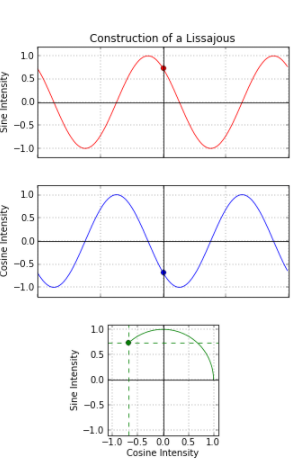
\includegraphics[width = 0.45\textwidth]{../img/Lissajous1.png}}
    \caption{Lissajous plot}
\end{figure}

\section*{Conclusion}
According to our Simulink modelling and TinkerCAD circuits, we can successfully control the printer head and measure its position to a suitable standard. After researching the status quo, we believe that the control methods (e.g. closed loop displacement control system) we have devised are acceptable for use in a mid-range 3D printer.

\begin{thebibliography}{00}
\bibitem{b1} 3D printing, how to obtain the best possible speeds, Chris Joel, https://www.3dprintersonlinestore.com/how-to-obtain-best-3d-printing-speed Accessed at 28-11-20 16:14:32
\bibitem{b2} Which Position Sensing Module Should You Use for Your RepRap 3D Printer?, Kalani Kirk Hausman, Richard Horne, https://www.dummies.com/computers/pcs/printers/which-position-sensing-module-should-you-use-for-your-reprap-3d-printer/ Accessed at 06-12-20 20:43:14
\bibitem{b3} Hall Effect Sensor, AspenCore Inc, https://www.electronics-tutorials.ws/electromagnetism/hall-effect.html Accessed at 06-12-20 20:51:19
\bibitem{b4} Hall Effect Sensor, AspenCore Inc, https://www.electronics-tutorials.ws/electromagnetism/hall-effect.html Accessed at 06-12-20 20:51:19, R. Portas, L. Colombel, https://www.iconopower.com/v/lem/coulometry.pdf Accessed at 06-12-20 20:56:43
\end{thebibliography}
\end{document}